% !TeX program = xelatex
% !TeX encoding = UTF-8
\documentclass[UTF8]{standalone}
\usepackage{amsmath,fourier,ctex,tikz}
\begin{document}
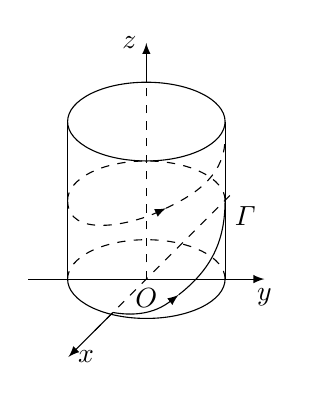
\begin{tikzpicture}
	\draw[dashed] (0,0) node[below] {$O$} -- (0,2.5);
	\draw[-latex] (0,2.5) --  (0,3) node[left] {$z$};
	\draw[-latex] (-1.5,0) -- (1.5,0) node[below] {$y$};
	\draw[-latex] (-135:0.6) -- ++ (-135:0.8) node[right] {$x$};
	\draw[dashed] (45:1.5) -- (-135:1);
	\draw[dashed] (1,0) arc [start angle=0, end angle=180, x radius=1, y radius=0.5];
	\draw (1,0) arc [start angle=0, end angle=-180, x radius=1, y radius=0.5];
	\draw (-1,0) -- ++ (0,2);
	\draw (1,0) -- ++ (0,2);
	\draw (1,2) arc [start angle=0, end angle=360, x radius=1, y radius=0.5];
	\draw[-latex] (-135:0.6)  to[out=-10,in=-142] (0.41,-0.2);
	\draw (0.41,-0.2) to[out=38,in=-90] (1,1);
	\draw[dashed] (1,1) arc [start angle=0, end angle=180, x radius=1, y radius=0.5];
	\draw[-latex,dashed] (-1,1) to[out=-90,in=-155] (0.25,0.9);
	\draw[dashed] (0.25,0.9) to[out=25,in=-90] (1,1.8);
	\node[right] at (1,0.8) {$\varGamma$};
\end{tikzpicture}
\end{document}